\documentclass[aspectratio=169,11pt]{beamer}
\usetheme{default}
\usefonttheme{serif}
\setbeamertemplate{navigation symbols}{}
\setbeamertemplate{itemize items}[circle]

\usepackage{tikz}
\usetikzlibrary{arrows.meta,positioning,calc}
\usepackage{pgfplots}
\pgfplotsset{compat=1.18}
\usepackage{booktabs}
\usepackage{xcolor}

\definecolor{ink}{HTML}{1F2328}
\definecolor{muted}{HTML}{6A737D}
\definecolor{faint}{HTML}{EEF0F3}
\definecolor{accent}{HTML}{1F6FEB}
\definecolor{good}{HTML}{1A7F37}
\definecolor{bad}{HTML}{CF222E}
\definecolor{warn}{HTML}{BF8700}
\definecolor{g1}{HTML}{C9D1D9}
\definecolor{g2}{HTML}{8C959F}
\definecolor{g3}{HTML}{57606A}

\setbeamercolor{normal text}{fg=ink}
\setbeamercolor{frametitle}{fg=ink}
\setbeamercolor{title}{fg=ink}
\setbeamercolor{structure}{fg=accent}
\setbeamercolor{block title}{bg=faint,fg=ink}
\setbeamercolor{block body}{bg=faint!50,fg=ink}
\setbeamerfont{frametitle}{size=\Large,series=\bfseries}

\setbeamertemplate{frametitle}{%
  \vspace{0.6em}\insertframetitle\par\vspace{-0.2em}%
  {\color{g1}\rule{\textwidth}{0.4pt}}}
\setbeamertemplate{footline}{%
  \hfill{\color{muted}\scriptsize\insertframenumber\,/\,\inserttotalframenumber}\hspace{1.2em}\vspace{0.8em}}

\newcommand{\src}[1]{\par\vfill\begin{minipage}{0.9\textwidth}\color{muted}\tiny #1\end{minipage}\vspace{-0.4em}}
\newcommand{\bignum}[3][ink]{{\color{#1}\fontsize{22}{24}\selectfont\bfseries #2}\\[2pt]{\color{muted}\small #3}}
\newcommand{\Source}{Ouro-1.4B (plain model), MATH train set, run 2026-11-05.}

\pgfplotsset{
  deck/.style={
    ybar, axis lines*=left, ymajorgrids, grid style={faint},
    tick label style={font=\footnotesize}, label style={font=\footnotesize},
    legend style={font=\footnotesize, draw=none, fill=none, legend columns=-1,
                  at={(0.5,1.03)}, anchor=south, /pgfplots/legend cell align=left},
    legend image code/.code={\draw[#1] (0cm,-0.1cm) rectangle (0.25cm,0.1cm);},
    enlarge x limits=0.15, xtick=data,
    every node near coord/.append style={font=\scriptsize, color=ink},
  },
}

\title{Does the change between loops tell us how hard a question is?}
\subtitle{LoopDelta, Stage 0 check on Ouro-1.4B}
\date{November 2026}

\begin{document}

%-------------------------------------------------------------
\begin{frame}[plain]
  \vspace{2em}
  {\color{muted}\small LoopDelta \;$\cdot$\; Stage 0 check \;$\cdot$\; Ouro-1.4B}\\[0.8em]
  {\LARGE\bfseries Does the cross-loop change $\Delta$ predict question difficulty?}\\[1.2em]
  {\color{muted} LoopDelta uses $\Delta$ to set per-question depth and to weight votes. Stage 0 tests whether $\Delta$ carries that signal.}
  \vspace{1.2em}
  \begin{block}{Answer: no}
    $\Delta$ tracks question length, not difficulty. Adaptive depth still has large headroom.
  \end{block}
  \vfill
  {\color{muted}\small November 2026}
\end{frame}

%-------------------------------------------------------------
\begin{frame}{The idea}
  Ouro runs 24 shared layers \textbf{4 times}. $\Delta$ = change in the KV cache between passes.
  \vspace{0.6em}

  \begin{columns}[T]
    \begin{column}{0.6\textwidth}
      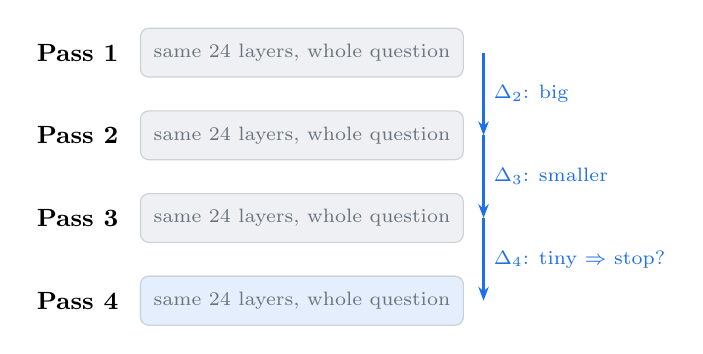
\begin{tikzpicture}[
          pass/.style={draw=g1, fill=faint, rounded corners=3pt, minimum width=4.1cm,
                       minimum height=0.62cm, font=\scriptsize\color{muted}},
          lab/.style={font=\small\bfseries, anchor=east}]
        \foreach \i in {1,2,3,4} {
          \node[pass] (p\i) at (0,-\i*1.05) {same 24 layers, whole question};
          \node[lab] at ($(p\i.west)+(-0.15,0)$) {Pass \i};
        }
        \node[pass, fill=accent!12] at (p4) {same 24 layers, whole question};
        \foreach \i/\d in {2/big, 3/smaller, 4/tiny $\Rightarrow$ stop?} {
          \pgfmathtruncatemacro{\j}{\i-1}
          \draw[-{Stealth[length=5pt]}, accent, thick] ($(p\j.east)+(0.25,0)$) -- ($(p\i.east)+(0.25,0)$)
            node[midway, right, font=\scriptsize, accent] {$\Delta_{\i}$: \d};
        }
      \end{tikzpicture}
    \end{column}
    \begin{column}{0.38\textwidth}
      \begin{block}{Use 1: depth}
        \small Stop once $\Delta$ is small.
      \end{block}
      \begin{block}{Use 2: voting}
        \small Weight solvers by $1/\Delta$.
      \end{block}
    \end{column}
  \end{columns}
  \src{$\Delta_t = \|X_t - X_{t-1}\|^2 / \|X_{t-1}\|^2$, $X\in\{K,V\}$, averaged over layers.}
\end{frame}

%-------------------------------------------------------------
\begin{frame}{What we ran}
  \begin{columns}[T]
    \begin{column}{0.48\textwidth}
      \begin{block}{A: prefill only}
        \small
        \begin{itemize}
          \item 1,000 MATH train questions, 200 per level 1--5
          \item Also run at 8 loops (2$\times$ training)
        \end{itemize}
      \end{block}
    \end{column}
    \begin{column}{0.48\textwidth}
      \begin{block}{B: generation}
        \small
        \begin{itemize}
          \item 300 questions, 60 per level, at 1, 2, 3 and 4 loops
          \item Per depth: 1 greedy + 4 sampled answers
          \item 6,000 graded answers
        \end{itemize}
      \end{block}
    \end{column}
  \end{columns}
  \vspace{1.1em}
  \begin{columns}[T]
    \begin{column}{0.24\textwidth}\bignum{1,000}{questions (A)}\end{column}
    \begin{column}{0.24\textwidth}\bignum{6,000}{answers (B)}\end{column}
    \begin{column}{0.24\textwidth}\bignum{5}{difficulty levels}\end{column}
    \begin{column}{0.24\textwidth}\bignum{1--4}{loops tested}\end{column}
  \end{columns}
\end{frame}

%-------------------------------------------------------------
\begin{frame}{Fewer loops is often enough}
  Most of the gain is 1 $\to$ 2 loops.
  \begin{center}
  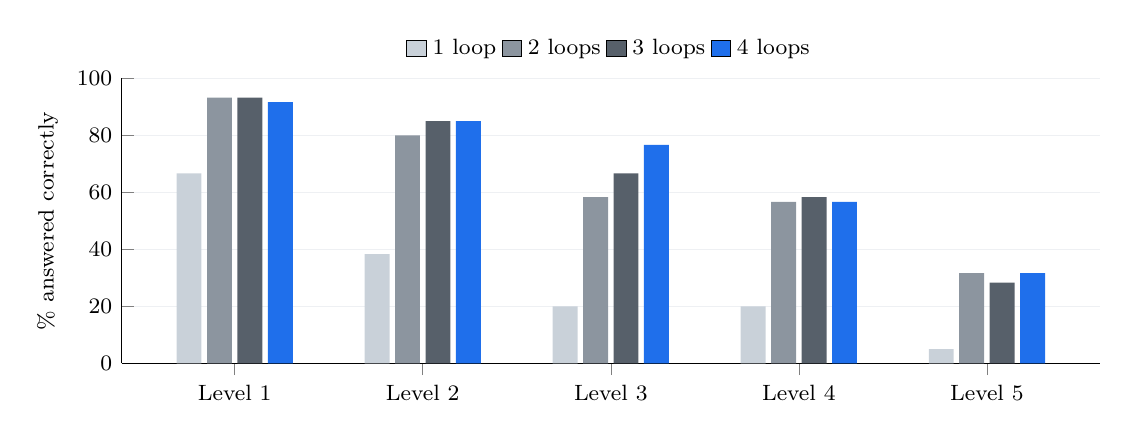
\begin{tikzpicture}
    \begin{axis}[deck, width=14cm, height=5.2cm, bar width=9pt, ymin=0, ymax=100,
        ylabel={\% answered correctly},
        symbolic x coords={Level 1, Level 2, Level 3, Level 4, Level 5}]
      \addplot[fill=g1, draw=none] coordinates {(Level 1,66.7) (Level 2,38.3) (Level 3,20) (Level 4,20) (Level 5,5)};
      \addplot[fill=g2, draw=none] coordinates {(Level 1,93.3) (Level 2,80) (Level 3,58.3) (Level 4,56.7) (Level 5,31.7)};
      \addplot[fill=g3, draw=none] coordinates {(Level 1,93.3) (Level 2,85) (Level 3,66.7) (Level 4,58.3) (Level 5,28.3)};
      \addplot[fill=accent, draw=none] coordinates {(Level 1,91.7) (Level 2,85) (Level 3,76.7) (Level 4,56.7) (Level 5,31.7)};
      \legend{1 loop, 2 loops, 3 loops, 4 loops}
    \end{axis}
  \end{tikzpicture}
  \end{center}
  \src{Greedy, 60 questions/level. Overall: 30\%, 64\%, 66\%, 68\%. \Source}
\end{frame}

%-------------------------------------------------------------
\begin{frame}{Minimum loops needed per question}
  70\% are solved by 2 loops.
  \begin{columns}[c]
    \begin{column}{0.58\textwidth}
      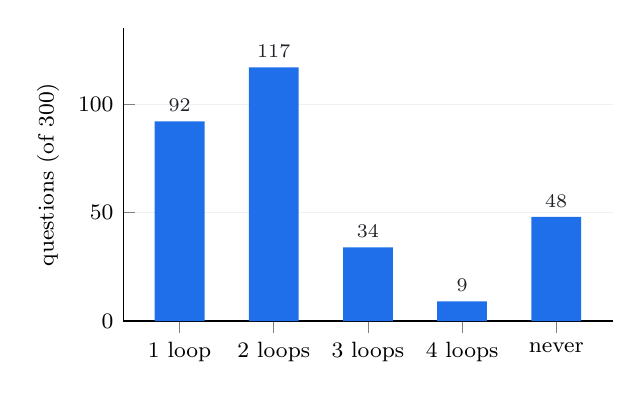
\begin{tikzpicture}
        \begin{axis}[deck, width=7.8cm, height=5.3cm, bar width=18pt, ymin=0, ymax=135,
            ylabel={questions (of 300)}, nodes near coords,
            symbolic x coords={1 loop, 2 loops, 3 loops, 4 loops, never}]
          \addplot[fill=accent, draw=none] coordinates {(1 loop,92) (2 loops,117) (3 loops,34) (4 loops,9) (never,48)};
        \end{axis}
      \end{tikzpicture}
    \end{column}
    \begin{column}{0.4\textwidth}
      \bignum[good]{77.8\%}{oracle depth picker}\\[1.2em]
      \bignum{68.0\%}{always 4 loops}\\[1.2em]
    \end{column}
  \end{columns}
  \src{Fewest loops with a correct greedy answer. Oracle on 153 held-out questions. \Source}
\end{frame}

%-------------------------------------------------------------
\begin{frame}{Test 1: does $\Delta$ track difficulty?}
  Only through question length.
  \begin{columns}[c]
    \begin{column}{0.6\textwidth}
      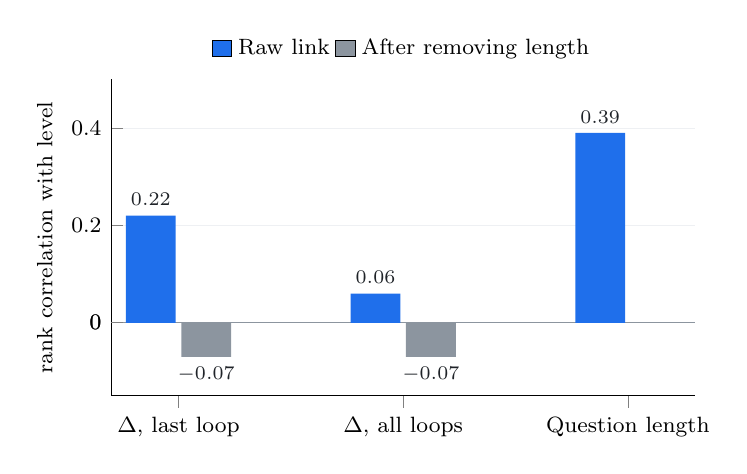
\begin{tikzpicture}
        \begin{axis}[deck, width=9cm, height=5.6cm, bar width=18pt, ymin=-0.15, ymax=0.5,
            ylabel={rank correlation with level}, nodes near coords,
            nodes near coords style={/pgf/number format/fixed, /pgf/number format/precision=2},
            symbolic x coords={{$\Delta$, last loop}, {$\Delta$, all loops}, {Question length}},
            extra y ticks={0}, extra y tick style={grid style={g2}}]
          \addplot[fill=accent, draw=none] coordinates {({$\Delta$, last loop},0.22) ({$\Delta$, all loops},0.06) ({Question length},0.39)};
          \addplot[fill=g2, draw=none] coordinates {({$\Delta$, last loop},-0.07) ({$\Delta$, all loops},-0.07)};
          \legend{Raw link, After removing length}
        \end{axis}
      \end{tikzpicture}
    \end{column}
    \begin{column}{0.38\textwidth}
      \begin{alertblock}{Takeaway}
        \small Given length, $\Delta$ adds nothing.
      \end{alertblock}
      \vspace{0.5em}
      {\small\color{muted} 8 loops: 0.23 raw, $-0.06$ partial.}
    \end{column}
  \end{columns}
  \src{Spearman with level, 1,000 questions, 4 loops. Partial = controlling for length. \Source}
\end{frame}

%-------------------------------------------------------------
\begin{frame}{Test 2: choosing depth}
  Question length does as well as $\Delta$.
  \vspace{0.8em}
  \begin{center}
  \renewcommand{\arraystretch}{1.25}
  \resizebox{0.75\textwidth}{!}{\begin{tabular}{lrl}
    \toprule
    \textbf{How depth is chosen} & \textbf{Accuracy} & \textbf{Verdict} \\
    \midrule
    Always 4 loops & 68.0\% & baseline \\
    Random & 67.5\% & chance \\
    Pick by $\Delta$ & 70.6\% & {\color{warn}+2.6} \\
    Pick by length & 70.6\% & {\color{good}\textbf{same as $\Delta$}} \\
    \midrule
    Oracle & 77.8\% & {\color{accent}ceiling} \\
    \bottomrule
  \end{tabular}}
  \end{center}
  \src{Greedy, thresholds fit on half, scored on 153 held-out questions (1 question = 0.65 pts). \Source}
\end{frame}

%-------------------------------------------------------------
\begin{frame}{Test 3: weighting votes}
  $\Delta$ barely beats chance at ranking right over wrong answers.
  \begin{columns}[c]
    \begin{column}{0.64\textwidth}
      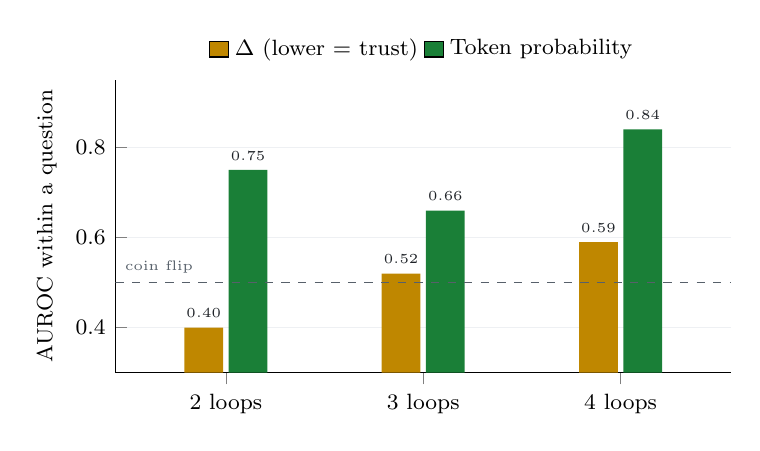
\begin{tikzpicture}
        \begin{axis}[deck, width=9.4cm, height=5.3cm, bar width=14pt, ymin=0.3, ymax=0.95,
            ylabel={AUROC within a question}, nodes near coords,
            nodes near coords style={/pgf/number format/fixed, /pgf/number format/fixed zerofill, /pgf/number format/precision=2},
            symbolic x coords={2 loops, 3 loops, 4 loops}, enlarge x limits=0.28,
            every node near coord/.append style={font=\tiny}]
          \addplot[fill=warn, draw=none] coordinates {(2 loops,0.40) (3 loops,0.52) (4 loops,0.59)};
          \addplot[fill=good, draw=none] coordinates {(2 loops,0.75) (3 loops,0.66) (4 loops,0.84)};
          \draw[dashed, g3] ({rel axis cs:0,0}|-{axis cs:2 loops,0.5}) -- ({rel axis cs:1,0}|-{axis cs:2 loops,0.5})
            node[pos=0.0, anchor=south west, font=\tiny, g3] {coin flip};
          \legend{$\Delta$ (lower = trust), Token probability}
        \end{axis}
      \end{tikzpicture}
    \end{column}
    \begin{column}{0.34\textwidth}
      {\small\textbf{Vote accuracy, 4 loops}}\\[0.3em]
      {\small\begin{tabular}{@{}lr@{}}
        \toprule
        Plain majority & 77.0\% \\
        {\color{warn}$\Delta$-weighted} & {\color{warn}76.3\%} \\
        Probability-weighted & 76.3\% \\
        \bottomrule
      \end{tabular}}\\[0.8em]
      {\footnotesize\color{muted} In 220 of 300 questions all 4 answers are right or all wrong, so weights can't change the vote.}\\[1em]
    \end{column}
  \end{columns}
  \src{AUROC over right/wrong answer pairs within a question (254--276 pairs from the $\sim$80 questions with mixed answers). Entropy $\approx$ token probability. \Source}
\end{frame}

%-------------------------------------------------------------
\begin{frame}{Side finding: voting}
  \begin{columns}[T]
    \begin{column}{0.55\textwidth}
      \textbf{Voting: 3 loops = 4 loops}\\[0.3em]
      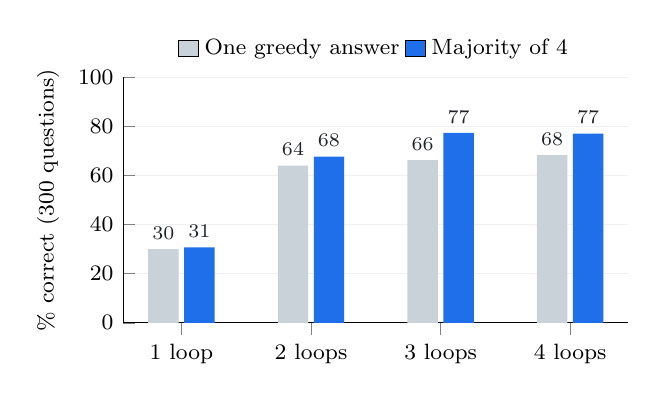
\begin{tikzpicture}
        \begin{axis}[deck, width=8cm, height=4.7cm, bar width=11pt, ymin=0, ymax=100,
            ylabel={\% correct (300 questions)}, nodes near coords,
            nodes near coords style={/pgf/number format/fixed, /pgf/number format/precision=0},
            symbolic x coords={1 loop, 2 loops, 3 loops, 4 loops}]
          \addplot[fill=g1, draw=none] coordinates {(1 loop,30) (2 loops,64) (3 loops,66.3) (4 loops,68.3)};
          \addplot[fill=accent, draw=none] coordinates {(1 loop,30.7) (2 loops,67.7) (3 loops,77.3) (4 loops,77.0)};
          \legend{One greedy answer, Majority of 4}
        \end{axis}
      \end{tikzpicture}\\
    \end{column}
    \begin{column}{0.42\textwidth}
      \bignum[good]{77.3\%}{vote, 3 loops}\\[1em]
      \bignum{77.0\%}{vote, 4 loops}\\[1em]
      {\small\color{muted} Voting adds $\sim$10 points from 3 loops on.}
    \end{column}
  \end{columns}
\end{frame}

%-------------------------------------------------------------
\begin{frame}{Verdict}
  \begin{center}
  \renewcommand{\arraystretch}{1.25}
  \resizebox{\textwidth}{!}{\begin{tabular}{lll}
    \toprule
    \textbf{Question} & \textbf{Evidence} & \textbf{Answer} \\
    \midrule
    Does $\Delta$ know difficulty? & 0.22 $\to$ $-0.07$ given length & {\color{bad}\textbf{only via length}} \\
    Does $\Delta$ pick depth well? & ties question length & {\color{bad}\textbf{no}} \\
    Does $\Delta$ pick good answers? & AUROC 0.40--0.59 & {\color{bad}\textbf{no}} \\
    Is adaptive depth worth it? & oracle 77.8\% vs 68.0\% & {\color{good}\textbf{yes}} \\
    \bottomrule
  \end{tabular}}
  \end{center}
  \vspace{0.6em}
  \begin{exampleblock}{Next}
    Drop $\Delta$. Test other depth signals on existing data: length, first-loop entropy, Ouro's exit gate.
  \end{exampleblock}
  \src{Caveats: one model, one dataset; 153 held-out questions; only 3 $\Delta$ values per question.}
\end{frame}

\end{document}
